\documentclass[1p]{elsarticle_modified}
%\bibliographystyle{elsarticle-num}

%\usepackage[colorlinks]{hyperref}
%\usepackage{abbrmath_seonhwa} %\Abb, \Ascr, \Acal ,\Abf, \Afrak
\usepackage{amsfonts}
\usepackage{amssymb}
\usepackage{amsmath}
\usepackage{amsthm}
\usepackage{scalefnt}
\usepackage{amsbsy}
\usepackage{kotex}
\usepackage{caption}
\usepackage{subfig}
\usepackage{color}
\usepackage{graphicx}
\usepackage{xcolor} %% white, black, red, green, blue, cyan, magenta, yellow
\usepackage{float}
\usepackage{setspace}
\usepackage{hyperref}

\usepackage{tikz}
\usetikzlibrary{arrows}

\usepackage{multirow}
\usepackage{array} % fixed length table
\usepackage{hhline}

%%%%%%%%%%%%%%%%%%%%%
\makeatletter
\renewcommand*\env@matrix[1][\arraystretch]{%
	\edef\arraystretch{#1}%
	\hskip -\arraycolsep
	\let\@ifnextchar\new@ifnextchar
	\array{*\c@MaxMatrixCols c}}
\makeatother %https://tex.stackexchange.com/questions/14071/how-can-i-increase-the-line-spacing-in-a-matrix
%%%%%%%%%%%%%%%

\usepackage[normalem]{ulem}

\newcommand{\msout}[1]{\ifmmode\text{\sout{\ensuremath{#1}}}\else\sout{#1}\fi}
%SOURCE: \msout is \stkout macro in https://tex.stackexchange.com/questions/20609/strikeout-in-math-mode

\newcommand{\cancel}[1]{
	\ifmmode
	{\color{red}\msout{#1}}
	\else
	{\color{red}\sout{#1}}
	\fi
}

\newcommand{\add}[1]{
	{\color{blue}\uwave{#1}}
}

\newcommand{\replace}[2]{
	\ifmmode
	{\color{red}\msout{#1}}{\color{blue}\uwave{#2}}
	\else
	{\color{red}\sout{#1}}{\color{blue}\uwave{#2}}
	\fi
}

\newcommand{\Sol}{\mathcal{S}} %segment
\newcommand{\D}{D} %diagram
\newcommand{\A}{\mathcal{A}} %arc


%%%%%%%%%%%%%%%%%%%%%%%%%%%%%5 test

\def\sl{\operatorname{\textup{SL}}(2,\Cbb)}
\def\psl{\operatorname{\textup{PSL}}(2,\Cbb)}
\def\quan{\mkern 1mu \triangleright \mkern 1mu}

\theoremstyle{definition}
\newtheorem{thm}{Theorem}[section]
\newtheorem{prop}[thm]{Proposition}
\newtheorem{lem}[thm]{Lemma}
\newtheorem{ques}[thm]{Question}
\newtheorem{cor}[thm]{Corollary}
\newtheorem{defn}[thm]{Definition}
\newtheorem{exam}[thm]{Example}
\newtheorem{rmk}[thm]{Remark}
\newtheorem{alg}[thm]{Algorithm}

\newcommand{\I}{\sqrt{-1}}
\begin{document}

%\begin{frontmatter}
%
%\title{Boundary parabolic representations of knots up to 8 crossings}
%
%%% Group authors per affiliation:
%\author{Yunhi Cho} 
%\address{Department of Mathematics, University of Seoul, Seoul, Korea}
%\ead{yhcho@uos.ac.kr}
%
%
%\author{Seonhwa Kim} %\fnref{s_kim}}
%\address{Center for Geometry and Physics, Institute for Basic Science, Pohang, 37673, Korea}
%\ead{ryeona17@ibs.re.kr}
%
%\author{Hyuk Kim}
%\address{Department of Mathematical Sciences, Seoul National University, Seoul 08826, Korea}
%\ead{hyukkim@snu.ac.kr}
%
%\author{Seokbeom Yoon}
%\address{Department of Mathematical Sciences, Seoul National University, Seoul, 08826,  Korea}
%\ead{sbyoon15@snu.ac.kr}
%
%\begin{abstract}
%We find all boundary parabolic representation of knots up to 8 crossings.
%
%\end{abstract}
%\begin{keyword}
%    \MSC[2010] 57M25 
%\end{keyword}
%
%\end{frontmatter}

%\linenumbers
%\tableofcontents
%
\newcommand\colored[1]{\textcolor{white}{\rule[-0.35ex]{0.8em}{1.4ex}}\kern-0.8em\color{red} #1}%
%\newcommand\colored[1]{\textcolor{white}{ #1}\kern-2.17ex	\textcolor{white}{ #1}\kern-1.81ex	\textcolor{white}{ #1}\kern-2.15ex\color{red}#1	}

{\Large $\underline{12a_{1141}~(K12a_{1141})}$}

\setlength{\tabcolsep}{10pt}
\renewcommand{\arraystretch}{1.6}
\vspace{1cm}\begin{tabular}{m{100pt}>{\centering\arraybackslash}m{274pt}}
\multirow{5}{120pt}{
	\centering
	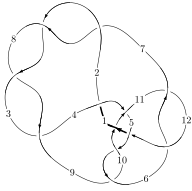
\includegraphics[width=112pt]{../../../GIT/diagram.site/Diagrams/png/1942_12a_1141.png}\\
\ \ \ A knot diagram\footnotemark}&
\allowdisplaybreaks
\textbf{Linearized knot diagam} \\
\cline{2-2}
 &
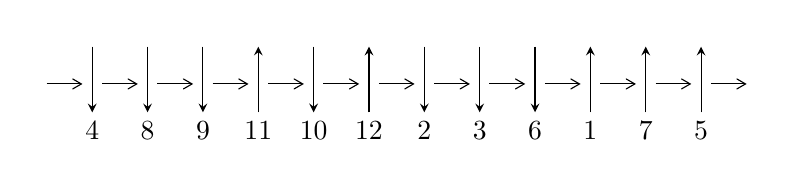
\begin{tikzpicture}[x=20pt, y=17pt]
	% nodes
	\node (C0) at (0, 0) {};
	\node (C1) at (1, 0) {};
	\node (C1U) at (1, +1) {};
	\node (C1D) at (1, -1) {4};

	\node (C2) at (2, 0) {};
	\node (C2U) at (2, +1) {};
	\node (C2D) at (2, -1) {8};

	\node (C3) at (3, 0) {};
	\node (C3U) at (3, +1) {};
	\node (C3D) at (3, -1) {9};

	\node (C4) at (4, 0) {};
	\node (C4U) at (4, +1) {};
	\node (C4D) at (4, -1) {11};

	\node (C5) at (5, 0) {};
	\node (C5U) at (5, +1) {};
	\node (C5D) at (5, -1) {10};

	\node (C6) at (6, 0) {};
	\node (C6U) at (6, +1) {};
	\node (C6D) at (6, -1) {12};

	\node (C7) at (7, 0) {};
	\node (C7U) at (7, +1) {};
	\node (C7D) at (7, -1) {2};

	\node (C8) at (8, 0) {};
	\node (C8U) at (8, +1) {};
	\node (C8D) at (8, -1) {3};

	\node (C9) at (9, 0) {};
	\node (C9U) at (9, +1) {};
	\node (C9D) at (9, -1) {6};

	\node (C10) at (10, 0) {};
	\node (C10U) at (10, +1) {};
	\node (C10D) at (10, -1) {1};

	\node (C11) at (11, 0) {};
	\node (C11U) at (11, +1) {};
	\node (C11D) at (11, -1) {7};

	\node (C12) at (12, 0) {};
	\node (C12U) at (12, +1) {};
	\node (C12D) at (12, -1) {5};
	\node (C13) at (13, 0) {};

	% arrows
	\draw[->,>={angle 60}]
	(C0) edge (C1) (C1) edge (C2) (C2) edge (C3) (C3) edge (C4) (C4) edge (C5) (C5) edge (C6) (C6) edge (C7) (C7) edge (C8) (C8) edge (C9) (C9) edge (C10) (C10) edge (C11) (C11) edge (C12) (C12) edge (C13) ;	\draw[->,>=stealth]
	(C1U) edge (C1D) (C2U) edge (C2D) (C3U) edge (C3D) (C4D) edge (C4U) (C5U) edge (C5D) (C6D) edge (C6U) (C7U) edge (C7D) (C8U) edge (C8D) (C9U) edge (C9D) (C10D) edge (C10U) (C11D) edge (C11U) (C12D) edge (C12U) ;
	\end{tikzpicture} \\
\hhline{~~} \\& 
\textbf{Solving Sequence} \\ \cline{2-2} 
 &
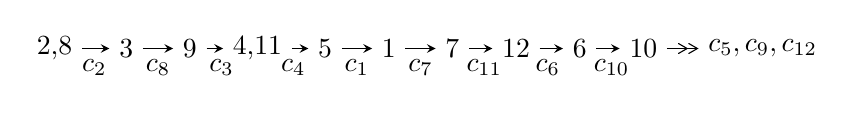
\begin{tikzpicture}[x=23pt, y=7pt]
	% node
	\node (A0) at (-1/8, 0) {2,8};
	\node (A1) at (1, 0) {3};
	\node (A2) at (2, 0) {9};
	\node (A3) at (49/16, 0) {4,11};
	\node (A4) at (33/8, 0) {5};
	\node (A5) at (41/8, 0) {1};
	\node (A6) at (49/8, 0) {7};
	\node (A7) at (57/8, 0) {12};
	\node (A8) at (65/8, 0) {6};
	\node (A9) at (73/8, 0) {10};
	\node (C1) at (1/2, -1) {$c_{2}$};
	\node (C2) at (3/2, -1) {$c_{8}$};
	\node (C3) at (5/2, -1) {$c_{3}$};
	\node (C4) at (29/8, -1) {$c_{4}$};
	\node (C5) at (37/8, -1) {$c_{1}$};
	\node (C6) at (45/8, -1) {$c_{7}$};
	\node (C7) at (53/8, -1) {$c_{11}$};
	\node (C8) at (61/8, -1) {$c_{6}$};
	\node (C9) at (69/8, -1) {$c_{10}$};
	\node (A10) at (11, 0) {$c_{5},c_{9},c_{12}$};

	% edge
	\draw[->,>=stealth]	
	(A0) edge (A1) (A1) edge (A2) (A2) edge (A3) (A3) edge (A4) (A4) edge (A5) (A5) edge (A6) (A6) edge (A7) (A7) edge (A8) (A8) edge (A9) ;
	\draw[->>,>={angle 60}]	
	(A9) edge (A10);
\end{tikzpicture} \\ 

\end{tabular} \\

\footnotetext{
The image of knot diagram is generated by the software ``\textbf{Draw programme}" developed by Andrew Bartholomew(\url{http://www.layer8.co.uk/maths/draw/index.htm\#Running-draw}), where we modified some parts for our purpose(\url{https://github.com/CATsTAILs/LinksPainter}).
}\phantom \\ \newline 
\centering \textbf{Ideals for irreducible components\footnotemark of $X_{\text{par}}$} 
 
\begin{align*}
I^u_{1}&=\langle 
-1.16393\times10^{80} u^{98}+1.96153\times10^{80} u^{97}+\cdots+1.45806\times10^{80} b-1.44154\times10^{81},\\
\phantom{I^u_{1}}&\phantom{= \langle  }2.69483\times10^{80} u^{98}+2.63977\times10^{81} u^{97}+\cdots+1.02064\times10^{81} a-2.84283\times10^{82},\;u^{99}+u^{98}+\cdots-18 u+7\rangle \\
I^u_{2}&=\langle 
- u^{14}+u^{13}+8 u^{12}-7 u^{11}-24 u^{10}+16 u^9+35 u^8-10 u^7-31 u^6-7 u^5+21 u^4+8 u^3-6 u^2+b-4 u+1,\\
\phantom{I^u_{2}}&\phantom{= \langle  }-2 u^{14}+u^{13}+\cdots+a+1,\\
\phantom{I^u_{2}}&\phantom{= \langle  }u^{16}-10 u^{14}+39 u^{12}+u^{11}-74 u^{10}-8 u^9+71 u^8+23 u^7-38 u^6-28 u^5+18 u^4+13 u^3-4 u^2-2 u+1\rangle \\
\\
\end{align*}
\raggedright * 2 irreducible components of $\dim_{\mathbb{C}}=0$, with total 115 representations.\\
\footnotetext{All coefficients of polynomials are rational numbers. But the coefficients are sometimes approximated in decimal forms when there is not enough margin.}
\newpage
\renewcommand{\arraystretch}{1}
\centering \section*{I. $I^u_{1}= \langle -1.16\times10^{80} u^{98}+1.96\times10^{80} u^{97}+\cdots+1.46\times10^{80} b-1.44\times10^{81},\;2.69\times10^{80} u^{98}+2.64\times10^{81} u^{97}+\cdots+1.02\times10^{81} a-2.84\times10^{82},\;u^{99}+u^{98}+\cdots-18 u+7 \rangle$}
\flushleft \textbf{(i) Arc colorings}\\
\begin{tabular}{m{7pt} m{180pt} m{7pt} m{180pt} }
\flushright $a_{2}=$&$\begin{pmatrix}1\\0\end{pmatrix}$ \\
\flushright $a_{8}=$&$\begin{pmatrix}0\\u\end{pmatrix}$ \\
\flushright $a_{3}=$&$\begin{pmatrix}1\\u^2\end{pmatrix}$ \\
\flushright $a_{9}=$&$\begin{pmatrix}- u\\- u^3+u\end{pmatrix}$ \\
\flushright $a_{4}=$&$\begin{pmatrix}- u^2+1\\- u^4+2 u^2\end{pmatrix}$ \\
\flushright $a_{11}=$&$\begin{pmatrix}-0.264033 u^{98}-2.58639 u^{97}+\cdots-24.9570 u+27.8534\\0.798272 u^{98}-1.34530 u^{97}+\cdots-18.0941 u+9.88675\end{pmatrix}$ \\
\flushright $a_{5}=$&$\begin{pmatrix}0.833020 u^{98}-1.92704 u^{97}+\cdots-27.1985 u+23.2113\\1.31877 u^{98}-1.84396 u^{97}+\cdots-38.6806 u+21.8148\end{pmatrix}$ \\
\flushright $a_{1}=$&$\begin{pmatrix}- u^6+3 u^4-2 u^2+1\\- u^8+4 u^6-4 u^4\end{pmatrix}$ \\
\flushright $a_{7}=$&$\begin{pmatrix}u\\u\end{pmatrix}$ \\
\flushright $a_{12}=$&$\begin{pmatrix}-0.00205647 u^{98}-2.51782 u^{97}+\cdots-29.1751 u+26.6019\\1.06025 u^{98}-1.27673 u^{97}+\cdots-22.3122 u+8.63527\end{pmatrix}$ \\
\flushright $a_{6}=$&$\begin{pmatrix}0.514009 u^{98}+1.64940 u^{97}+\cdots+14.5324 u-20.0768\\-0.502672 u^{98}+1.10075 u^{97}+\cdots+15.7291 u-8.88776\end{pmatrix}$ \\
\flushright $a_{10}=$&$\begin{pmatrix}0.370327 u^{98}-2.17342 u^{97}+\cdots-29.7554 u+24.1137\\1.00004 u^{98}-1.94343 u^{97}+\cdots-28.8770 u+14.8644\end{pmatrix}$\\&\end{tabular}
\flushleft \textbf{(ii) Obstruction class $= -1$}\\~\\
\flushleft \textbf{(iii) Cusp Shapes $= 4.35878 u^{98}+7.93657 u^{97}+\cdots+50.8346 u-78.6235$}\\~\\
\newpage\renewcommand{\arraystretch}{1}
\flushleft \textbf{(iv) u-Polynomials at the component}\newline \\
\begin{tabular}{m{50pt}|m{274pt}}
Crossings & \hspace{64pt}u-Polynomials at each crossing \\
\hline $$\begin{aligned}c_{1}\end{aligned}$$&$\begin{aligned}
&u^{99}-23 u^{98}+\cdots+738442 u-80017
\end{aligned}$\\
\hline $$\begin{aligned}c_{2},c_{3},c_{7}\\c_{8}\end{aligned}$$&$\begin{aligned}
&u^{99}+u^{98}+\cdots-18 u+7
\end{aligned}$\\
\hline $$\begin{aligned}c_{4}\end{aligned}$$&$\begin{aligned}
&u^{99}+2 u^{97}+\cdots+270 u+25
\end{aligned}$\\
\hline $$\begin{aligned}c_{5},c_{9}\end{aligned}$$&$\begin{aligned}
&u^{99}+2 u^{98}+\cdots+1662 u+229
\end{aligned}$\\
\hline $$\begin{aligned}c_{6},c_{11}\end{aligned}$$&$\begin{aligned}
&u^{99}+u^{98}+\cdots- u+7
\end{aligned}$\\
\hline $$\begin{aligned}c_{10}\end{aligned}$$&$\begin{aligned}
&u^{99}+13 u^{98}+\cdots-4180 u-1361
\end{aligned}$\\
\hline $$\begin{aligned}c_{12}\end{aligned}$$&$\begin{aligned}
&u^{99}-5 u^{98}+\cdots-3 u+5
\end{aligned}$\\
\hline
\end{tabular}\\~\\
\newpage\renewcommand{\arraystretch}{1}
\flushleft \textbf{(v) Riley Polynomials at the component}\newline \\
\begin{tabular}{m{50pt}|m{274pt}}
Crossings & \hspace{64pt}Riley Polynomials at each crossing \\
\hline $$\begin{aligned}c_{1}\end{aligned}$$&$\begin{aligned}
&y^{99}+19 y^{98}+\cdots-55556666826 y-6402720289
\end{aligned}$\\
\hline $$\begin{aligned}c_{2},c_{3},c_{7}\\c_{8}\end{aligned}$$&$\begin{aligned}
&y^{99}-113 y^{98}+\cdots+954 y-49
\end{aligned}$\\
\hline $$\begin{aligned}c_{4}\end{aligned}$$&$\begin{aligned}
&y^{99}+4 y^{98}+\cdots+11450 y-625
\end{aligned}$\\
\hline $$\begin{aligned}c_{5},c_{9}\end{aligned}$$&$\begin{aligned}
&y^{99}+64 y^{98}+\cdots+1987766 y-52441
\end{aligned}$\\
\hline $$\begin{aligned}c_{6},c_{11}\end{aligned}$$&$\begin{aligned}
&y^{99}+63 y^{98}+\cdots-1595 y-49
\end{aligned}$\\
\hline $$\begin{aligned}c_{10}\end{aligned}$$&$\begin{aligned}
&y^{99}-25 y^{98}+\cdots+92281126 y-1852321
\end{aligned}$\\
\hline $$\begin{aligned}c_{12}\end{aligned}$$&$\begin{aligned}
&y^{99}-5 y^{98}+\cdots-591 y-25
\end{aligned}$\\
\hline
\end{tabular}\\~\\
\newpage\flushleft \textbf{(vi) Complex Volumes and Cusp Shapes}
$$\begin{array}{c|c|c}  
\text{Solutions to }I^u_{1}& \I (\text{vol} + \sqrt{-1}CS) & \text{Cusp shape}\\
 \hline 
\begin{aligned}
u &= -0.763291 + 0.609745 I \\
a &= -0.310082 - 0.171201 I \\
b &= -0.749409 + 0.925641 I\end{aligned}
 & \phantom{-}0.86700 + 4.61216 I & \phantom{-0.000000 } 0 \\ \hline\begin{aligned}
u &= -0.763291 - 0.609745 I \\
a &= -0.310082 + 0.171201 I \\
b &= -0.749409 - 0.925641 I\end{aligned}
 & \phantom{-}0.86700 - 4.61216 I & \phantom{-0.000000 } 0 \\ \hline\begin{aligned}
u &= \phantom{-}0.691941 + 0.585463 I \\
a &= \phantom{-}1.024370 - 0.210352 I \\
b &= \phantom{-}1.40382 + 1.37236 I\end{aligned}
 & \phantom{-}0.9782 - 14.1492 I & \phantom{-0.000000 } 0 \\ \hline\begin{aligned}
u &= \phantom{-}0.691941 - 0.585463 I \\
a &= \phantom{-}1.024370 + 0.210352 I \\
b &= \phantom{-}1.40382 - 1.37236 I\end{aligned}
 & \phantom{-}0.9782 + 14.1492 I & \phantom{-0.000000 } 0 \\ \hline\begin{aligned}
u &= \phantom{-}0.798193 + 0.428389 I \\
a &= -0.247703 - 0.269691 I \\
b &= -0.613093 - 0.868425 I\end{aligned}
 & -0.09955 - 3.40884 I & \phantom{-0.000000 } 0 \\ \hline\begin{aligned}
u &= \phantom{-}0.798193 - 0.428389 I \\
a &= -0.247703 + 0.269691 I \\
b &= -0.613093 + 0.868425 I\end{aligned}
 & -0.09955 + 3.40884 I & \phantom{-0.000000 } 0 \\ \hline\begin{aligned}
u &= \phantom{-}0.437870 + 0.789230 I \\
a &= \phantom{-}0.101251 + 0.317677 I \\
b &= -0.503643 - 0.222196 I\end{aligned}
 & \phantom{-}3.61622 - 2.57236 I & \phantom{-0.000000 } 0 \\ \hline\begin{aligned}
u &= \phantom{-}0.437870 - 0.789230 I \\
a &= \phantom{-}0.101251 - 0.317677 I \\
b &= -0.503643 + 0.222196 I\end{aligned}
 & \phantom{-}3.61622 + 2.57236 I & \phantom{-0.000000 } 0 \\ \hline\begin{aligned}
u &= \phantom{-}0.848923 + 0.087013 I \\
a &= -0.592659 - 0.955005 I \\
b &= -0.231461 + 0.462338 I\end{aligned}
 & -5.69841 + 1.85582 I & \phantom{-0.000000 } 0 \\ \hline\begin{aligned}
u &= \phantom{-}0.848923 - 0.087013 I \\
a &= -0.592659 + 0.955005 I \\
b &= -0.231461 - 0.462338 I\end{aligned}
 & -5.69841 - 1.85582 I & \phantom{-0.000000 } 0\\
 \hline 
 \end{array}$$\newpage$$\begin{array}{c|c|c}  
\text{Solutions to }I^u_{1}& \I (\text{vol} + \sqrt{-1}CS) & \text{Cusp shape}\\
 \hline 
\begin{aligned}
u &= -0.649236 + 0.536213 I \\
a &= \phantom{-}1.146540 + 0.196143 I \\
b &= \phantom{-}1.61665 - 1.19536 I\end{aligned}
 & -2.81830 + 7.75472 I & \phantom{-0.000000 } 0 \\ \hline\begin{aligned}
u &= -0.649236 - 0.536213 I \\
a &= \phantom{-}1.146540 - 0.196143 I \\
b &= \phantom{-}1.61665 + 1.19536 I\end{aligned}
 & -2.81830 - 7.75472 I & \phantom{-0.000000 } 0 \\ \hline\begin{aligned}
u &= -1.142900 + 0.201687 I \\
a &= -0.506272 + 0.893053 I \\
b &= \phantom{-}0.1036290 + 0.0001587 I\end{aligned}
 & -2.15673 - 6.65249 I & \phantom{-0.000000 } 0 \\ \hline\begin{aligned}
u &= -1.142900 - 0.201687 I \\
a &= -0.506272 - 0.893053 I \\
b &= \phantom{-}0.1036290 - 0.0001587 I\end{aligned}
 & -2.15673 + 6.65249 I & \phantom{-0.000000 } 0 \\ \hline\begin{aligned}
u &= -0.609435 + 0.533021 I \\
a &= -1.47973 + 0.57722 I \\
b &= -0.114393 + 1.380160 I\end{aligned}
 & \phantom{-}4.41559 + 7.48924 I & \phantom{-0.000000 } 0 \\ \hline\begin{aligned}
u &= -0.609435 - 0.533021 I \\
a &= -1.47973 - 0.57722 I \\
b &= -0.114393 - 1.380160 I\end{aligned}
 & \phantom{-}4.41559 - 7.48924 I & \phantom{-0.000000 } 0 \\ \hline\begin{aligned}
u &= \phantom{-}0.676022 + 0.428807 I \\
a &= -1.39804 + 0.28148 I \\
b &= -1.24437 - 1.50203 I\end{aligned}
 & -1.43426 - 5.86382 I & \phantom{-0.000000 } 0 \\ \hline\begin{aligned}
u &= \phantom{-}0.676022 - 0.428807 I \\
a &= -1.39804 - 0.28148 I \\
b &= -1.24437 + 1.50203 I\end{aligned}
 & -1.43426 + 5.86382 I & \phantom{-0.000000 } 0 \\ \hline\begin{aligned}
u &= -0.728898 + 0.301402 I \\
a &= \phantom{-}0.463149 - 1.182220 I \\
b &= -0.714291 - 0.035123 I\end{aligned}
 & -2.26210 - 0.32498 I & \phantom{-0.000000 } 0 \\ \hline\begin{aligned}
u &= -0.728898 - 0.301402 I \\
a &= \phantom{-}0.463149 + 1.182220 I \\
b &= -0.714291 + 0.035123 I\end{aligned}
 & -2.26210 + 0.32498 I & \phantom{-0.000000 } 0\\
 \hline 
 \end{array}$$\newpage$$\begin{array}{c|c|c}  
\text{Solutions to }I^u_{1}& \I (\text{vol} + \sqrt{-1}CS) & \text{Cusp shape}\\
 \hline 
\begin{aligned}
u &= \phantom{-}0.502985 + 0.582942 I \\
a &= \phantom{-}0.746369 - 0.416319 I \\
b &= \phantom{-}0.767382 + 0.220139 I\end{aligned}
 & \phantom{-}3.96912 - 1.96998 I & \phantom{-0.000000 } 0 \\ \hline\begin{aligned}
u &= \phantom{-}0.502985 - 0.582942 I \\
a &= \phantom{-}0.746369 + 0.416319 I \\
b &= \phantom{-}0.767382 - 0.220139 I\end{aligned}
 & \phantom{-}3.96912 + 1.96998 I & \phantom{-0.000000 } 0 \\ \hline\begin{aligned}
u &= \phantom{-}0.488561 + 0.594766 I \\
a &= \phantom{-}0.188342 - 0.610285 I \\
b &= \phantom{-}0.679847 - 0.474605 I\end{aligned}
 & \phantom{-}4.01500 - 2.06533 I & \phantom{-0.000000 } 0 \\ \hline\begin{aligned}
u &= \phantom{-}0.488561 - 0.594766 I \\
a &= \phantom{-}0.188342 + 0.610285 I \\
b &= \phantom{-}0.679847 + 0.474605 I\end{aligned}
 & \phantom{-}4.01500 + 2.06533 I & \phantom{-0.000000 } 0 \\ \hline\begin{aligned}
u &= \phantom{-}0.620258 + 0.414743 I \\
a &= -0.983477 - 0.837263 I \\
b &= -0.367877 - 1.128180 I\end{aligned}
 & \phantom{-}0.15736 - 3.84244 I & \phantom{-0.000000 -}0. + 7.19805 I \\ \hline\begin{aligned}
u &= \phantom{-}0.620258 - 0.414743 I \\
a &= -0.983477 + 0.837263 I \\
b &= -0.367877 + 1.128180 I\end{aligned}
 & \phantom{-}0.15736 + 3.84244 I & \phantom{-0.000000 } 0. - 7.19805 I \\ \hline\begin{aligned}
u &= \phantom{-}0.250868 + 0.687008 I \\
a &= -1.180340 - 0.709707 I \\
b &= \phantom{-}0.716050 - 0.942890 I\end{aligned}
 & \phantom{-}2.28768 + 9.87518 I & -2.00000 - 5.33704 I \\ \hline\begin{aligned}
u &= \phantom{-}0.250868 - 0.687008 I \\
a &= -1.180340 + 0.709707 I \\
b &= \phantom{-}0.716050 + 0.942890 I\end{aligned}
 & \phantom{-}2.28768 - 9.87518 I & -2.00000 + 5.33704 I \\ \hline\begin{aligned}
u &= -0.114104 + 0.710742 I \\
a &= \phantom{-}1.021980 + 0.034819 I \\
b &= -0.272551 - 0.242795 I\end{aligned}
 & \phantom{-}2.77279 - 0.19088 I & \phantom{-}4.76195 - 1.33883 I \\ \hline\begin{aligned}
u &= -0.114104 - 0.710742 I \\
a &= \phantom{-}1.021980 - 0.034819 I \\
b &= -0.272551 + 0.242795 I\end{aligned}
 & \phantom{-}2.77279 + 0.19088 I & \phantom{-}4.76195 + 1.33883 I\\
 \hline 
 \end{array}$$\newpage$$\begin{array}{c|c|c}  
\text{Solutions to }I^u_{1}& \I (\text{vol} + \sqrt{-1}CS) & \text{Cusp shape}\\
 \hline 
\begin{aligned}
u &= -0.574003 + 0.422917 I \\
a &= -0.98239 - 1.03631 I \\
b &= -1.56531 + 0.74752 I\end{aligned}
 & -2.25497 + 2.06352 I & -5.88569 - 4.07985 I \\ \hline\begin{aligned}
u &= -0.574003 - 0.422917 I \\
a &= -0.98239 + 1.03631 I \\
b &= -1.56531 - 0.74752 I\end{aligned}
 & -2.25497 - 2.06352 I & -5.88569 + 4.07985 I \\ \hline\begin{aligned}
u &= -0.551944 + 0.442603 I \\
a &= \phantom{-}0.142792 - 0.247167 I \\
b &= \phantom{-}0.69382 - 1.76142 I\end{aligned}
 & \phantom{-}1.87885 + 5.04729 I & \phantom{-0.000000 } 0. - 8.53052 I \\ \hline\begin{aligned}
u &= -0.551944 - 0.442603 I \\
a &= \phantom{-}0.142792 + 0.247167 I \\
b &= \phantom{-}0.69382 + 1.76142 I\end{aligned}
 & \phantom{-}1.87885 - 5.04729 I & \phantom{-0.000000 -}0. + 8.53052 I \\ \hline\begin{aligned}
u &= -1.297430 + 0.245162 I \\
a &= -0.724683 - 0.405345 I \\
b &= -0.553294 + 0.342994 I\end{aligned}
 & -1.84376 + 6.35965 I & \phantom{-0.000000 } 0 \\ \hline\begin{aligned}
u &= -1.297430 - 0.245162 I \\
a &= -0.724683 + 0.405345 I \\
b &= -0.553294 - 0.342994 I\end{aligned}
 & -1.84376 - 6.35965 I & \phantom{-0.000000 } 0 \\ \hline\begin{aligned}
u &= -0.330304 + 0.573316 I \\
a &= \phantom{-}0.761223 + 0.313103 I \\
b &= \phantom{-}0.33905 - 1.40088 I\end{aligned}
 & \phantom{-}5.23430 - 3.68890 I & \phantom{-}2.98854 + 1.79364 I \\ \hline\begin{aligned}
u &= -0.330304 - 0.573316 I \\
a &= \phantom{-}0.761223 - 0.313103 I \\
b &= \phantom{-}0.33905 + 1.40088 I\end{aligned}
 & \phantom{-}5.23430 + 3.68890 I & \phantom{-}2.98854 - 1.79364 I \\ \hline\begin{aligned}
u &= -0.270684 + 0.587647 I \\
a &= -1.15217 + 1.17890 I \\
b &= \phantom{-}0.638102 + 0.968916 I\end{aligned}
 & -1.71656 - 3.90788 I & -3.38936 + 3.68440 I \\ \hline\begin{aligned}
u &= -0.270684 - 0.587647 I \\
a &= -1.15217 - 1.17890 I \\
b &= \phantom{-}0.638102 - 0.968916 I\end{aligned}
 & -1.71656 + 3.90788 I & -3.38936 - 3.68440 I\\
 \hline 
 \end{array}$$\newpage$$\begin{array}{c|c|c}  
\text{Solutions to }I^u_{1}& \I (\text{vol} + \sqrt{-1}CS) & \text{Cusp shape}\\
 \hline 
\begin{aligned}
u &= \phantom{-}0.521611 + 0.357512 I \\
a &= \phantom{-}0.69052 + 1.77803 I \\
b &= -1.005600 - 0.390867 I\end{aligned}
 & -2.87449 - 1.28088 I & -2.04294 + 6.38847 I \\ \hline\begin{aligned}
u &= \phantom{-}0.521611 - 0.357512 I \\
a &= \phantom{-}0.69052 - 1.77803 I \\
b &= -1.005600 + 0.390867 I\end{aligned}
 & -2.87449 + 1.28088 I & -2.04294 - 6.38847 I \\ \hline\begin{aligned}
u &= -0.569395 + 0.213633 I \\
a &= \phantom{-}0.815353 - 0.538900 I \\
b &= -0.037666 - 0.231193 I\end{aligned}
 & -1.071210 + 0.471534 I & -7.90805 - 1.67970 I \\ \hline\begin{aligned}
u &= -0.569395 - 0.213633 I \\
a &= \phantom{-}0.815353 + 0.538900 I \\
b &= -0.037666 + 0.231193 I\end{aligned}
 & -1.071210 - 0.471534 I & -7.90805 + 1.67970 I \\ \hline\begin{aligned}
u &= -0.419265 + 0.424814 I \\
a &= -2.13162 + 1.24115 I \\
b &= -0.358198 + 0.662173 I\end{aligned}
 & \phantom{-}2.28522 - 1.94327 I & \phantom{-}3.21298 - 1.03946 I \\ \hline\begin{aligned}
u &= -0.419265 - 0.424814 I \\
a &= -2.13162 - 1.24115 I \\
b &= -0.358198 - 0.662173 I\end{aligned}
 & \phantom{-}2.28522 + 1.94327 I & \phantom{-}3.21298 + 1.03946 I \\ \hline\begin{aligned}
u &= \phantom{-}0.517050 + 0.296886 I \\
a &= \phantom{-}0.934378 + 0.341756 I \\
b &= \phantom{-}1.56636 + 1.33611 I\end{aligned}
 & \phantom{-}0.87417 + 1.73334 I & -4.33449 + 2.25502 I \\ \hline\begin{aligned}
u &= \phantom{-}0.517050 - 0.296886 I \\
a &= \phantom{-}0.934378 - 0.341756 I \\
b &= \phantom{-}1.56636 - 1.33611 I\end{aligned}
 & \phantom{-}0.87417 - 1.73334 I & -4.33449 - 2.25502 I \\ \hline\begin{aligned}
u &= \phantom{-}1.42400 + 0.08728 I \\
a &= \phantom{-}1.61066 + 0.70366 I \\
b &= \phantom{-}0.96811 + 1.12630 I\end{aligned}
 & -0.26486 + 1.46630 I & \phantom{-0.000000 } 0 \\ \hline\begin{aligned}
u &= \phantom{-}1.42400 - 0.08728 I \\
a &= \phantom{-}1.61066 - 0.70366 I \\
b &= \phantom{-}0.96811 - 1.12630 I\end{aligned}
 & -0.26486 - 1.46630 I & \phantom{-0.000000 } 0\\
 \hline 
 \end{array}$$\newpage$$\begin{array}{c|c|c}  
\text{Solutions to }I^u_{1}& \I (\text{vol} + \sqrt{-1}CS) & \text{Cusp shape}\\
 \hline 
\begin{aligned}
u &= \phantom{-}1.44232 + 0.02930 I \\
a &= -1.03789 - 1.40791 I \\
b &= -0.879871 - 0.773001 I\end{aligned}
 & -6.73733 + 2.03033 I & \phantom{-0.000000 } 0 \\ \hline\begin{aligned}
u &= \phantom{-}1.44232 - 0.02930 I \\
a &= -1.03789 + 1.40791 I \\
b &= -0.879871 + 0.773001 I\end{aligned}
 & -6.73733 - 2.03033 I & \phantom{-0.000000 } 0 \\ \hline\begin{aligned}
u &= -0.303479 + 0.431708 I \\
a &= \phantom{-}0.86305 - 1.28776 I \\
b &= -0.986240 - 0.387244 I\end{aligned}
 & -1.52675 + 0.96711 I & -4.03573 - 4.34958 I \\ \hline\begin{aligned}
u &= -0.303479 - 0.431708 I \\
a &= \phantom{-}0.86305 + 1.28776 I \\
b &= -0.986240 + 0.387244 I\end{aligned}
 & -1.52675 - 0.96711 I & -4.03573 + 4.34958 I \\ \hline\begin{aligned}
u &= -1.48799\phantom{ +0.000000I} \\
a &= \phantom{-}2.09639\phantom{ +0.000000I} \\
b &= \phantom{-}1.68145\phantom{ +0.000000I}\end{aligned}
 & -4.04626\phantom{ +0.000000I} & \phantom{-0.000000 } 0 \\ \hline\begin{aligned}
u &= \phantom{-}0.494977 + 0.033800 I \\
a &= \phantom{-}1.76169 - 1.98879 I \\
b &= \phantom{-}0.439062 - 0.955413 I\end{aligned}
 & \phantom{-}0.87319 - 3.26894 I & -5.13325 + 7.07926 I \\ \hline\begin{aligned}
u &= \phantom{-}0.494977 - 0.033800 I \\
a &= \phantom{-}1.76169 + 1.98879 I \\
b &= \phantom{-}0.439062 + 0.955413 I\end{aligned}
 & \phantom{-}0.87319 + 3.26894 I & -5.13325 - 7.07926 I \\ \hline\begin{aligned}
u &= \phantom{-}0.220361 + 0.439245 I \\
a &= \phantom{-}0.959569 - 0.061026 I \\
b &= \phantom{-}0.380950 + 0.742407 I\end{aligned}
 & \phantom{-}1.31423 + 0.82561 I & \phantom{-}3.50137 - 0.32849 I \\ \hline\begin{aligned}
u &= \phantom{-}0.220361 - 0.439245 I \\
a &= \phantom{-}0.959569 + 0.061026 I \\
b &= \phantom{-}0.380950 - 0.742407 I\end{aligned}
 & \phantom{-}1.31423 - 0.82561 I & \phantom{-}3.50137 + 0.32849 I \\ \hline\begin{aligned}
u &= -1.51425 + 0.17065 I \\
a &= \phantom{-}0.527100 + 1.191720 I \\
b &= \phantom{-}0.597586 + 0.935450 I\end{aligned}
 & -2.57936 + 4.78942 I & \phantom{-0.000000 } 0\\
 \hline 
 \end{array}$$\newpage$$\begin{array}{c|c|c}  
\text{Solutions to }I^u_{1}& \I (\text{vol} + \sqrt{-1}CS) & \text{Cusp shape}\\
 \hline 
\begin{aligned}
u &= -1.51425 - 0.17065 I \\
a &= \phantom{-}0.527100 - 1.191720 I \\
b &= \phantom{-}0.597586 - 0.935450 I\end{aligned}
 & -2.57936 - 4.78942 I & \phantom{-0.000000 } 0 \\ \hline\begin{aligned}
u &= \phantom{-}0.101860 + 0.460295 I \\
a &= \phantom{-}1.84322 - 0.11187 I \\
b &= -0.595286 + 0.892959 I\end{aligned}
 & \phantom{-}0.12875 + 2.77820 I & -1.87617 - 4.60612 I \\ \hline\begin{aligned}
u &= \phantom{-}0.101860 - 0.460295 I \\
a &= \phantom{-}1.84322 + 0.11187 I \\
b &= -0.595286 - 0.892959 I\end{aligned}
 & \phantom{-}0.12875 - 2.77820 I & -1.87617 + 4.60612 I \\ \hline\begin{aligned}
u &= \phantom{-}1.52610 + 0.09330 I \\
a &= -1.80851 - 0.49814 I \\
b &= -1.356600 + 0.129572 I\end{aligned}
 & -4.27161 + 0.25928 I & \phantom{-0.000000 } 0 \\ \hline\begin{aligned}
u &= \phantom{-}1.52610 - 0.09330 I \\
a &= -1.80851 + 0.49814 I \\
b &= -1.356600 - 0.129572 I\end{aligned}
 & -4.27161 - 0.25928 I & \phantom{-0.000000 } 0 \\ \hline\begin{aligned}
u &= -1.52712 + 0.15738 I \\
a &= \phantom{-}1.48245 + 0.37484 I \\
b &= \phantom{-}1.130290 + 0.082284 I\end{aligned}
 & -2.74425 + 4.58226 I & \phantom{-0.000000 } 0 \\ \hline\begin{aligned}
u &= -1.52712 - 0.15738 I \\
a &= \phantom{-}1.48245 - 0.37484 I \\
b &= \phantom{-}1.130290 - 0.082284 I\end{aligned}
 & -2.74425 - 4.58226 I & \phantom{-0.000000 } 0 \\ \hline\begin{aligned}
u &= -1.55819 + 0.03781 I \\
a &= \phantom{-}1.51013 - 1.40745 I \\
b &= \phantom{-}0.796484 - 1.079400 I\end{aligned}
 & -6.20517 - 2.93963 I & \phantom{-0.000000 } 0 \\ \hline\begin{aligned}
u &= -1.55819 - 0.03781 I \\
a &= \phantom{-}1.51013 + 1.40745 I \\
b &= \phantom{-}0.796484 + 1.079400 I\end{aligned}
 & -6.20517 + 2.93963 I & \phantom{-0.000000 } 0 \\ \hline\begin{aligned}
u &= -1.55895 + 0.08512 I \\
a &= \phantom{-}2.84299 - 1.47477 I \\
b &= \phantom{-}2.79322 - 2.03600 I\end{aligned}
 & -6.23677 - 0.35234 I & \phantom{-0.000000 } 0\\
 \hline 
 \end{array}$$\newpage$$\begin{array}{c|c|c}  
\text{Solutions to }I^u_{1}& \I (\text{vol} + \sqrt{-1}CS) & \text{Cusp shape}\\
 \hline 
\begin{aligned}
u &= -1.55895 - 0.08512 I \\
a &= \phantom{-}2.84299 + 1.47477 I \\
b &= \phantom{-}2.79322 + 2.03600 I\end{aligned}
 & -6.23677 + 0.35234 I & \phantom{-0.000000 } 0 \\ \hline\begin{aligned}
u &= -1.56027 + 0.09761 I \\
a &= -0.825260 - 0.038446 I \\
b &= -1.04023 + 1.11745 I\end{aligned}
 & -9.98972 + 2.89332 I & \phantom{-0.000000 } 0 \\ \hline\begin{aligned}
u &= -1.56027 - 0.09761 I \\
a &= -0.825260 + 0.038446 I \\
b &= -1.04023 - 1.11745 I\end{aligned}
 & -9.98972 - 2.89332 I & \phantom{-0.000000 } 0 \\ \hline\begin{aligned}
u &= \phantom{-}1.55972 + 0.12130 I \\
a &= \phantom{-}1.70559 + 2.08880 I \\
b &= \phantom{-}1.57167 + 2.85062 I\end{aligned}
 & -5.26165 - 7.05580 I & \phantom{-0.000000 } 0 \\ \hline\begin{aligned}
u &= \phantom{-}1.55972 - 0.12130 I \\
a &= \phantom{-}1.70559 - 2.08880 I \\
b &= \phantom{-}1.57167 - 2.85062 I\end{aligned}
 & -5.26165 + 7.05580 I & \phantom{-0.000000 } 0 \\ \hline\begin{aligned}
u &= \phantom{-}1.56570 + 0.07807 I \\
a &= \phantom{-}0.749210 + 0.562591 I \\
b &= \phantom{-}0.286823 + 0.284697 I\end{aligned}
 & -8.34824 - 1.63671 I & \phantom{-0.000000 } 0 \\ \hline\begin{aligned}
u &= \phantom{-}1.56570 - 0.07807 I \\
a &= \phantom{-}0.749210 - 0.562591 I \\
b &= \phantom{-}0.286823 - 0.284697 I\end{aligned}
 & -8.34824 + 1.63671 I & \phantom{-0.000000 } 0 \\ \hline\begin{aligned}
u &= \phantom{-}1.56598 + 0.11409 I \\
a &= -2.55571 - 0.12395 I \\
b &= -2.26156 - 1.03244 I\end{aligned}
 & -9.50202 - 3.97617 I & \phantom{-0.000000 } 0 \\ \hline\begin{aligned}
u &= \phantom{-}1.56598 - 0.11409 I \\
a &= -2.55571 + 0.12395 I \\
b &= -2.26156 + 1.03244 I\end{aligned}
 & -9.50202 + 3.97617 I & \phantom{-0.000000 } 0 \\ \hline\begin{aligned}
u &= \phantom{-}1.57047 + 0.15448 I \\
a &= -1.42059 - 1.23113 I \\
b &= -0.545692 - 1.202280 I\end{aligned}
 & -2.90241 - 9.99401 I & \phantom{-0.000000 } 0\\
 \hline 
 \end{array}$$\newpage$$\begin{array}{c|c|c}  
\text{Solutions to }I^u_{1}& \I (\text{vol} + \sqrt{-1}CS) & \text{Cusp shape}\\
 \hline 
\begin{aligned}
u &= \phantom{-}1.57047 - 0.15448 I \\
a &= -1.42059 + 1.23113 I \\
b &= -0.545692 + 1.202280 I\end{aligned}
 & -2.90241 + 9.99401 I & \phantom{-0.000000 } 0 \\ \hline\begin{aligned}
u &= -1.57507 + 0.11656 I \\
a &= -1.61810 + 1.13603 I \\
b &= -1.18957 + 1.06359 I\end{aligned}
 & -7.26990 + 5.77422 I & \phantom{-0.000000 } 0 \\ \hline\begin{aligned}
u &= -1.57507 - 0.11656 I \\
a &= -1.61810 - 1.13603 I \\
b &= -1.18957 - 1.06359 I\end{aligned}
 & -7.26990 - 5.77422 I & \phantom{-0.000000 } 0 \\ \hline\begin{aligned}
u &= \phantom{-}1.58482 + 0.15976 I \\
a &= \phantom{-}2.79031 + 0.46182 I \\
b &= \phantom{-}2.55704 + 1.24136 I\end{aligned}
 & -10.3375 - 10.3262 I & \phantom{-0.000000 } 0 \\ \hline\begin{aligned}
u &= \phantom{-}1.58482 - 0.15976 I \\
a &= \phantom{-}2.79031 - 0.46182 I \\
b &= \phantom{-}2.55704 - 1.24136 I\end{aligned}
 & -10.3375 + 10.3262 I & \phantom{-0.000000 } 0 \\ \hline\begin{aligned}
u &= -1.59587 + 0.12411 I \\
a &= -2.45389 + 1.03531 I \\
b &= -1.93276 + 1.84915 I\end{aligned}
 & -9.15520 + 7.91610 I & \phantom{-0.000000 } 0 \\ \hline\begin{aligned}
u &= -1.59587 - 0.12411 I \\
a &= -2.45389 - 1.03531 I \\
b &= -1.93276 - 1.84915 I\end{aligned}
 & -9.15520 - 7.91610 I & \phantom{-0.000000 } 0 \\ \hline\begin{aligned}
u &= \phantom{-}1.60647 + 0.08510 I \\
a &= -0.542163 + 0.210261 I \\
b &= -0.890760 - 0.619723 I\end{aligned}
 & -10.24050 - 1.11922 I & \phantom{-0.000000 } 0 \\ \hline\begin{aligned}
u &= \phantom{-}1.60647 - 0.08510 I \\
a &= -0.542163 - 0.210261 I \\
b &= -0.890760 + 0.619723 I\end{aligned}
 & -10.24050 + 1.11922 I & \phantom{-0.000000 } 0 \\ \hline\begin{aligned}
u &= -1.60022 + 0.17865 I \\
a &= \phantom{-}2.45649 - 0.73425 I \\
b &= \phantom{-}2.13417 - 1.63116 I\end{aligned}
 & -6.7302 + 17.0060 I & \phantom{-0.000000 } 0\\
 \hline 
 \end{array}$$\newpage$$\begin{array}{c|c|c}  
\text{Solutions to }I^u_{1}& \I (\text{vol} + \sqrt{-1}CS) & \text{Cusp shape}\\
 \hline 
\begin{aligned}
u &= -1.60022 - 0.17865 I \\
a &= \phantom{-}2.45649 + 0.73425 I \\
b &= \phantom{-}2.13417 + 1.63116 I\end{aligned}
 & -6.7302 - 17.0060 I & \phantom{-0.000000 } 0 \\ \hline\begin{aligned}
u &= -1.62129 + 0.02269 I \\
a &= -0.422405 - 0.828882 I \\
b &= -0.28613 - 1.67040 I\end{aligned}
 & -14.1221 - 1.4415 I & \phantom{-0.000000 } 0 \\ \hline\begin{aligned}
u &= -1.62129 - 0.02269 I \\
a &= -0.422405 + 0.828882 I \\
b &= -0.28613 + 1.67040 I\end{aligned}
 & -14.1221 + 1.4415 I & \phantom{-0.000000 } 0 \\ \hline\begin{aligned}
u &= \phantom{-}1.61475 + 0.19360 I \\
a &= -1.46104 - 0.59865 I \\
b &= -1.35349 - 1.38366 I\end{aligned}
 & -7.10456 - 7.68717 I & \phantom{-0.000000 } 0 \\ \hline\begin{aligned}
u &= \phantom{-}1.61475 - 0.19360 I \\
a &= -1.46104 + 0.59865 I \\
b &= -1.35349 + 1.38366 I\end{aligned}
 & -7.10456 + 7.68717 I & \phantom{-0.000000 } 0 \\ \hline\begin{aligned}
u &= -1.62392 + 0.13743 I \\
a &= -1.56203 + 0.90007 I \\
b &= -1.47911 + 1.38232 I\end{aligned}
 & -8.31409 + 5.62806 I & \phantom{-0.000000 } 0 \\ \hline\begin{aligned}
u &= -1.62392 - 0.13743 I \\
a &= -1.56203 - 0.90007 I \\
b &= -1.47911 - 1.38232 I\end{aligned}
 & -8.31409 - 5.62806 I & \phantom{-0.000000 } 0 \\ \hline\begin{aligned}
u &= \phantom{-}1.67170 + 0.00590 I \\
a &= -0.075885 - 0.586017 I \\
b &= \phantom{-}0.107620 - 1.333890 I\end{aligned}
 & -11.85680 - 6.44606 I & \phantom{-0.000000 } 0 \\ \hline\begin{aligned}
u &= \phantom{-}1.67170 - 0.00590 I \\
a &= -0.075885 + 0.586017 I \\
b &= \phantom{-}0.107620 + 1.333890 I\end{aligned}
 & -11.85680 + 6.44606 I & \phantom{-0.000000 } 0\\
 \hline 
 \end{array}$$\newpage\newpage\renewcommand{\arraystretch}{1}
\centering \section*{II. $I^u_{2}= \langle - u^{14}+u^{13}+\cdots+b+1,\;-2 u^{14}+u^{13}+\cdots+a+1,\;u^{16}-10 u^{14}+\cdots-2 u+1 \rangle$}
\flushleft \textbf{(i) Arc colorings}\\
\begin{tabular}{m{7pt} m{180pt} m{7pt} m{180pt} }
\flushright $a_{2}=$&$\begin{pmatrix}1\\0\end{pmatrix}$ \\
\flushright $a_{8}=$&$\begin{pmatrix}0\\u\end{pmatrix}$ \\
\flushright $a_{3}=$&$\begin{pmatrix}1\\u^2\end{pmatrix}$ \\
\flushright $a_{9}=$&$\begin{pmatrix}- u\\- u^3+u\end{pmatrix}$ \\
\flushright $a_{4}=$&$\begin{pmatrix}- u^2+1\\- u^4+2 u^2\end{pmatrix}$ \\
\flushright $a_{11}=$&$\begin{pmatrix}2 u^{14}- u^{13}+\cdots+8 u-1\\u^{14}- u^{13}+\cdots+4 u-1\end{pmatrix}$ \\
\flushright $a_{5}=$&$\begin{pmatrix}- u^{15}+9 u^{13}+\cdots-3 u-1\\u^{12}-7 u^{10}+17 u^8+u^7-16 u^6-5 u^5+5 u^4+7 u^3-2 u^2-3 u\end{pmatrix}$ \\
\flushright $a_{1}=$&$\begin{pmatrix}- u^6+3 u^4-2 u^2+1\\- u^8+4 u^6-4 u^4\end{pmatrix}$ \\
\flushright $a_{7}=$&$\begin{pmatrix}u\\u\end{pmatrix}$ \\
\flushright $a_{12}=$&$\begin{pmatrix}u^{14}- u^{13}+\cdots+10 u^2+6 u\\- u^{13}+7 u^{11}-17 u^9-2 u^8+16 u^7+9 u^6-5 u^5-11 u^4+u^3+2 u^2+2 u\end{pmatrix}$ \\
\flushright $a_{6}=$&$\begin{pmatrix}- u^{15}+u^{14}+\cdots+2 u+1\\u^{15}+u^{14}+\cdots-2 u+1\end{pmatrix}$ \\
\flushright $a_{10}=$&$\begin{pmatrix}2 u^{14}- u^{13}+\cdots+6 u-1\\u^{14}- u^{13}+\cdots+4 u-1\end{pmatrix}$\\&\end{tabular}
\flushleft \textbf{(ii) Obstruction class $= 1$}\\~\\
\flushleft \textbf{(iii) Cusp Shapes $= u^{15}-3 u^{13}- u^{12}-18 u^{11}+7 u^{10}+94 u^9-11 u^8-143 u^7-19 u^6+84 u^5+58 u^4-38 u^3-33 u^2+11 u-1$}\\~\\
\newpage\renewcommand{\arraystretch}{1}
\flushleft \textbf{(iv) u-Polynomials at the component}\newline \\
\begin{tabular}{m{50pt}|m{274pt}}
Crossings & \hspace{64pt}u-Polynomials at each crossing \\
\hline $$\begin{aligned}c_{1}\end{aligned}$$&$\begin{aligned}
&u^{16}+4 u^{15}+\cdots-2 u+1
\end{aligned}$\\
\hline $$\begin{aligned}c_{2},c_{3}\end{aligned}$$&$\begin{aligned}
&u^{16}-10 u^{14}+\cdots-2 u+1
\end{aligned}$\\
\hline $$\begin{aligned}c_{4}\end{aligned}$$&$\begin{aligned}
&u^{16}+u^{15}+\cdots+2 u^3+1
\end{aligned}$\\
\hline $$\begin{aligned}c_{5}\end{aligned}$$&$\begin{aligned}
&u^{16}+u^{15}+\cdots+8 u^2+1
\end{aligned}$\\
\hline $$\begin{aligned}c_{6}\end{aligned}$$&$\begin{aligned}
&u^{16}+8 u^{14}+\cdots- u+1
\end{aligned}$\\
\hline $$\begin{aligned}c_{7},c_{8}\end{aligned}$$&$\begin{aligned}
&u^{16}-10 u^{14}+\cdots+2 u+1
\end{aligned}$\\
\hline $$\begin{aligned}c_{9}\end{aligned}$$&$\begin{aligned}
&u^{16}- u^{15}+\cdots+8 u^2+1
\end{aligned}$\\
\hline $$\begin{aligned}c_{10}\end{aligned}$$&$\begin{aligned}
&u^{16}-4 u^{14}+\cdots+8 u+1
\end{aligned}$\\
\hline $$\begin{aligned}c_{11}\end{aligned}$$&$\begin{aligned}
&u^{16}+8 u^{14}+\cdots+u+1
\end{aligned}$\\
\hline $$\begin{aligned}c_{12}\end{aligned}$$&$\begin{aligned}
&u^{16}-2 u^{13}-2 u^{12}+u^{11}+u^9+3 u^8-2 u^7+u^6+u^5- u^4+u^3- u^2- u+1
\end{aligned}$\\
\hline
\end{tabular}\\~\\
\newpage\renewcommand{\arraystretch}{1}
\flushleft \textbf{(v) Riley Polynomials at the component}\newline \\
\begin{tabular}{m{50pt}|m{274pt}}
Crossings & \hspace{64pt}Riley Polynomials at each crossing \\
\hline $$\begin{aligned}c_{1}\end{aligned}$$&$\begin{aligned}
&y^{16}+4 y^{15}+\cdots+12 y+1
\end{aligned}$\\
\hline $$\begin{aligned}c_{2},c_{3},c_{7}\\c_{8}\end{aligned}$$&$\begin{aligned}
&y^{16}-20 y^{15}+\cdots-12 y+1
\end{aligned}$\\
\hline $$\begin{aligned}c_{4}\end{aligned}$$&$\begin{aligned}
&y^{16}-3 y^{15}+\cdots-4 y^2+1
\end{aligned}$\\
\hline $$\begin{aligned}c_{5},c_{9}\end{aligned}$$&$\begin{aligned}
&y^{16}+13 y^{15}+\cdots+16 y+1
\end{aligned}$\\
\hline $$\begin{aligned}c_{6},c_{11}\end{aligned}$$&$\begin{aligned}
&y^{16}+16 y^{15}+\cdots+13 y+1
\end{aligned}$\\
\hline $$\begin{aligned}c_{10}\end{aligned}$$&$\begin{aligned}
&y^{16}-8 y^{15}+\cdots-8 y+1
\end{aligned}$\\
\hline $$\begin{aligned}c_{12}\end{aligned}$$&$\begin{aligned}
&y^{16}-4 y^{14}+\cdots-3 y+1
\end{aligned}$\\
\hline
\end{tabular}\\~\\
\newpage\flushleft \textbf{(vi) Complex Volumes and Cusp Shapes}
$$\begin{array}{c|c|c}  
\text{Solutions to }I^u_{2}& \I (\text{vol} + \sqrt{-1}CS) & \text{Cusp shape}\\
 \hline 
\begin{aligned}
u &= \phantom{-}0.749888 + 0.412737 I \\
a &= -0.482981 - 0.157116 I \\
b &= -0.57933 - 1.35783 I\end{aligned}
 & -0.31642 - 4.80216 I & -4.28190 + 8.53963 I \\ \hline\begin{aligned}
u &= \phantom{-}0.749888 - 0.412737 I \\
a &= -0.482981 + 0.157116 I \\
b &= -0.57933 + 1.35783 I\end{aligned}
 & -0.31642 + 4.80216 I & -4.28190 - 8.53963 I \\ \hline\begin{aligned}
u &= -0.441315 + 0.700895 I \\
a &= \phantom{-}0.028510 - 0.642080 I \\
b &= -0.644596 - 0.091812 I\end{aligned}
 & \phantom{-}3.29668 + 2.36445 I & -7.72275 - 1.32048 I \\ \hline\begin{aligned}
u &= -0.441315 - 0.700895 I \\
a &= \phantom{-}0.028510 + 0.642080 I \\
b &= -0.644596 + 0.091812 I\end{aligned}
 & \phantom{-}3.29668 - 2.36445 I & -7.72275 + 1.32048 I \\ \hline\begin{aligned}
u &= -0.569717 + 0.232049 I \\
a &= -0.10645 - 2.03638 I \\
b &= -1.200940 + 0.301920 I\end{aligned}
 & -3.44134 + 0.81986 I & -12.20354 + 0.25953 I \\ \hline\begin{aligned}
u &= -0.569717 - 0.232049 I \\
a &= -0.10645 + 2.03638 I \\
b &= -1.200940 - 0.301920 I\end{aligned}
 & -3.44134 - 0.81986 I & -12.20354 - 0.25953 I \\ \hline\begin{aligned}
u &= \phantom{-}1.48473 + 0.16212 I \\
a &= -0.320775 + 1.110710 I \\
b &= -0.230819 + 0.697084 I\end{aligned}
 & -2.82368 - 5.27538 I & -7.16301 + 8.89431 I \\ \hline\begin{aligned}
u &= \phantom{-}1.48473 - 0.16212 I \\
a &= -0.320775 - 1.110710 I \\
b &= -0.230819 - 0.697084 I\end{aligned}
 & -2.82368 + 5.27538 I & -7.16301 - 8.89431 I \\ \hline\begin{aligned}
u &= -1.52213 + 0.04939 I \\
a &= \phantom{-}2.32971 - 1.33467 I \\
b &= \phantom{-}1.97084 - 0.94365 I\end{aligned}
 & -5.10540 - 1.62333 I & -2.28629 + 4.04054 I \\ \hline\begin{aligned}
u &= -1.52213 - 0.04939 I \\
a &= \phantom{-}2.32971 + 1.33467 I \\
b &= \phantom{-}1.97084 + 0.94365 I\end{aligned}
 & -5.10540 + 1.62333 I & -2.28629 - 4.04054 I\\
 \hline 
 \end{array}$$\newpage$$\begin{array}{c|c|c}  
\text{Solutions to }I^u_{2}& \I (\text{vol} + \sqrt{-1}CS) & \text{Cusp shape}\\
 \hline 
\begin{aligned}
u &= \phantom{-}1.58491 + 0.07036 I \\
a &= -1.102130 + 0.179111 I \\
b &= -1.25975 - 0.84936 I\end{aligned}
 & -10.91500 - 1.94360 I & -11.86525 + 1.00527 I \\ \hline\begin{aligned}
u &= \phantom{-}1.58491 - 0.07036 I \\
a &= -1.102130 - 0.179111 I \\
b &= -1.25975 + 0.84936 I\end{aligned}
 & -10.91500 + 1.94360 I & -11.86525 - 1.00527 I \\ \hline\begin{aligned}
u &= \phantom{-}0.324777 + 0.221310 I \\
a &= \phantom{-}2.90404 + 1.73077 I \\
b &= \phantom{-}0.936104 + 0.903034 I\end{aligned}
 & \phantom{-}1.32598 + 2.48939 I & -0.39288 - 3.29934 I \\ \hline\begin{aligned}
u &= \phantom{-}0.324777 - 0.221310 I \\
a &= \phantom{-}2.90404 - 1.73077 I \\
b &= \phantom{-}0.936104 - 0.903034 I\end{aligned}
 & \phantom{-}1.32598 - 2.48939 I & -0.39288 + 3.29934 I \\ \hline\begin{aligned}
u &= -1.61115 + 0.13456 I \\
a &= -1.74992 + 1.16607 I \\
b &= -1.49151 + 1.86069 I\end{aligned}
 & -8.33978 + 6.95567 I & -6.08440 - 5.77311 I \\ \hline\begin{aligned}
u &= -1.61115 - 0.13456 I \\
a &= -1.74992 - 1.16607 I \\
b &= -1.49151 - 1.86069 I\end{aligned}
 & -8.33978 - 6.95567 I & -6.08440 + 5.77311 I\\
 \hline 
 \end{array}$$\newpage
\newpage\renewcommand{\arraystretch}{1}
\centering \section*{ III. u-Polynomials}
\begin{tabular}{m{50pt}|m{274pt}}
Crossings & \hspace{64pt}u-Polynomials at each crossing \\
\hline $$\begin{aligned}c_{1}\end{aligned}$$&$\begin{aligned}
&(u^{16}+4 u^{15}+\cdots-2 u+1)(u^{99}-23 u^{98}+\cdots+738442 u-80017)
\end{aligned}$\\
\hline $$\begin{aligned}c_{2},c_{3}\end{aligned}$$&$\begin{aligned}
&(u^{16}-10 u^{14}+\cdots-2 u+1)(u^{99}+u^{98}+\cdots-18 u+7)
\end{aligned}$\\
\hline $$\begin{aligned}c_{4}\end{aligned}$$&$\begin{aligned}
&(u^{16}+u^{15}+\cdots+2 u^3+1)(u^{99}+2 u^{97}+\cdots+270 u+25)
\end{aligned}$\\
\hline $$\begin{aligned}c_{5}\end{aligned}$$&$\begin{aligned}
&(u^{16}+u^{15}+\cdots+8 u^2+1)(u^{99}+2 u^{98}+\cdots+1662 u+229)
\end{aligned}$\\
\hline $$\begin{aligned}c_{6}\end{aligned}$$&$\begin{aligned}
&(u^{16}+8 u^{14}+\cdots- u+1)(u^{99}+u^{98}+\cdots- u+7)
\end{aligned}$\\
\hline $$\begin{aligned}c_{7},c_{8}\end{aligned}$$&$\begin{aligned}
&(u^{16}-10 u^{14}+\cdots+2 u+1)(u^{99}+u^{98}+\cdots-18 u+7)
\end{aligned}$\\
\hline $$\begin{aligned}c_{9}\end{aligned}$$&$\begin{aligned}
&(u^{16}- u^{15}+\cdots+8 u^2+1)(u^{99}+2 u^{98}+\cdots+1662 u+229)
\end{aligned}$\\
\hline $$\begin{aligned}c_{10}\end{aligned}$$&$\begin{aligned}
&(u^{16}-4 u^{14}+\cdots+8 u+1)(u^{99}+13 u^{98}+\cdots-4180 u-1361)
\end{aligned}$\\
\hline $$\begin{aligned}c_{11}\end{aligned}$$&$\begin{aligned}
&(u^{16}+8 u^{14}+\cdots+u+1)(u^{99}+u^{98}+\cdots- u+7)
\end{aligned}$\\
\hline $$\begin{aligned}c_{12}\end{aligned}$$&$\begin{aligned}
&(u^{16}-2 u^{13}-2 u^{12}+u^{11}+u^9+3 u^8-2 u^7+u^6+u^5- u^4+u^3- u^2- u+1)\\
&\cdot(u^{99}-5 u^{98}+\cdots-3 u+5)
\end{aligned}$\\
\hline
\end{tabular}\newpage\renewcommand{\arraystretch}{1}
\centering \section*{ IV. Riley Polynomials}
\begin{tabular}{m{50pt}|m{274pt}}
Crossings & \hspace{64pt}Riley Polynomials at each crossing \\
\hline $$\begin{aligned}c_{1}\end{aligned}$$&$\begin{aligned}
&(y^{16}+4 y^{15}+\cdots+12 y+1)\\
&\cdot(y^{99}+19 y^{98}+\cdots-55556666826 y-6402720289)
\end{aligned}$\\
\hline $$\begin{aligned}c_{2},c_{3},c_{7}\\c_{8}\end{aligned}$$&$\begin{aligned}
&(y^{16}-20 y^{15}+\cdots-12 y+1)(y^{99}-113 y^{98}+\cdots+954 y-49)
\end{aligned}$\\
\hline $$\begin{aligned}c_{4}\end{aligned}$$&$\begin{aligned}
&(y^{16}-3 y^{15}+\cdots-4 y^2+1)(y^{99}+4 y^{98}+\cdots+11450 y-625)
\end{aligned}$\\
\hline $$\begin{aligned}c_{5},c_{9}\end{aligned}$$&$\begin{aligned}
&(y^{16}+13 y^{15}+\cdots+16 y+1)(y^{99}+64 y^{98}+\cdots+1987766 y-52441)
\end{aligned}$\\
\hline $$\begin{aligned}c_{6},c_{11}\end{aligned}$$&$\begin{aligned}
&(y^{16}+16 y^{15}+\cdots+13 y+1)(y^{99}+63 y^{98}+\cdots-1595 y-49)
\end{aligned}$\\
\hline $$\begin{aligned}c_{10}\end{aligned}$$&$\begin{aligned}
&(y^{16}-8 y^{15}+\cdots-8 y+1)\\
&\cdot(y^{99}-25 y^{98}+\cdots+92281126 y-1852321)
\end{aligned}$\\
\hline $$\begin{aligned}c_{12}\end{aligned}$$&$\begin{aligned}
&(y^{16}-4 y^{14}+\cdots-3 y+1)(y^{99}-5 y^{98}+\cdots-591 y-25)
\end{aligned}$\\
\hline
\end{tabular}
\vskip 2pc
\end{document}